\PassOptionsToPackage{utf8}{inputenc}
\documentclass{bioinfo}
\copyrightyear{2020} \pubyear{2020}
\newcommand{\R}{\mathbb{R}}

\access{Advance Access Publication Date: Day Month Year}
\appnotes{ISMB 2020}
\begin{document}
\firstpage{1}

\subtitle{Subject Section}

\title[short Title]{
CoRAE: Concreate Relaxations Autoencoder for Differentiable Gene Selection and Pan-Cancer Classification
% Pan-Cancer Feature Selection and Classification Reveals Key RNAs for Cancers
% Epigenetic Landscape Using Pan-Cancer Feature Selection and Classification
}
\author[Sample \textit{et~al}.]{Abdullah Al Mamun\, and Ananda Mondal*}
% $^{\text{\sfb 1,}*}$, Co-Author\,$^{\text{\sfb 2}}$ and Co-Author\,$^{\text{\sfb 2,}*}$}

\address
{
% $^{\text{\sf 1}}$
School of Computing and Information Sciences, Miami, US \\
% $^{\text{\sf 2}}$
% Department, Institution, City, Post Code,Country.
}

\corresp{$^\ast$To whom correspondence should be addressed.}

\history{Received on XXXXX; revised on XXXXX; accepted on XXXXX}

\editor{Associate Editor: XXXXXXX}

\abstract{\textbf{Motivation:} 
%Selecting an important feature is a critical study in omics data classification. Feature selection aims to select less number of important features that will increase accuracy and decrease the cost of data classification. Due to having high-dimension with a low number of samples, classification models encountered over-fitting problem with TCGA multi-omics data. Therefore, the demand for feature selection methods that are capable of selecting a few numbers of important features is felt. 
%In recent years, autoencoder has been used to select significant features to increase the classification performance. However, the standard autoencoder is not able to provide the original features. In this paper, we are introducing a novel global feature selection method based on concrete relaxation discrete random variable selection,  which efficiently identifies a subset of most significant features that have more contribution in data classification and reconstruction. The proposed method is a variation of standard autoencoder where a concrete feature selection layer as the encoder and a standard neural network as decoder are used. During training the model, a predefined temperature of the feature selection layer is steadily decreased which allows the model to learn a used-specified number of discrete features. During testing the model, only selected features can be used in the decoder to reconstruct the input.
\\
\textbf{Results:} 
%We evaluated CoRAE on coding and non-coding gene expression datasets where it significantly outperforms state-of-the-art methods for identifying top 100 coding and non-coding genes for distinguishing 33 different cancers. Later, selected gene expression shows a significant classification performance up to $99\%$. The proposed method can be implemented by adding a few lines of code to the standard autoencoder.\\

\textbf{Availability:} Source code and toy dataset can be found in https://github.com/pwaabdullah/MyPhD.git\\
\textbf{Contact:} \href{amondal@fiu.edu}{amondal@fiu.edu}\\
\textbf{Supplementary information:} Supplementary data are available at \textit{Bioinformatics}
online.}

\maketitle

\section{Introduction}
%The big issue of recent omics data is large number of features compared to the number of samples available. Among all the features, few might be meaningful to separate the samples which belongs to different classes and rest of these are either irrelevent, redundant, or noise \citep{pirgazi2019efficient}. During classification or clustering the high dimensional data, irrelevent features creates unnecessary computational complexities and decrease the performance. Therefore, it is essential to identify the most relavent features that would has high contribution in classificaiton/clustering task. During feature selection process, redundent features are removed because there is a subset of features that carries approximate similar information. In similarly fashion, noise features that provide no information about labels are also be removed from the database. Thus, only relevent features will be remain that will increase the efficiency of any classification/clustering task. 
\section{Materials and Methods}
\subsection{Gene Expression}
To validated the proposed idea, TCGA RNAseq cancer (n=9566) and clinical samples for 33 cancers were downloaded from UCSC Xena database (https://xenabrowser.net). TCGA processed raw RNAseq data using Illumina HiSeq 2000 RNA sequencing platform where per-gene normalized abundance estimation were calculated with FPKM method. RNASeq normalized counts were then log transformed after adding a constant of 1.  Later UCSC re-processed using GENCODE v23 transcript annotation to quantify protein coding() and non-coding transcripts() expression \cite{harrow2006gencode}. Coding genes refers to mRNA whereas non-coding genes refers to miRNA, and long non-coding RNA (lncRNA) in this experiment. To improve the focus on individual feature selection, we separated mRNA, miRNA and lncRNA expression from combined database using mirBase and TANRIC[] database those provids standard list of miRNAs and lncRNAs. Another important reason of performing experiment on individual RNA types is because their expression level is different. The number of mRNA, miRNA, and lncRNA are 18731, 602, 12309 respectively. We merged all the cancer samples for individual RNA types for further experiment. Each row is mapped to a unique Ensemble ID, and each column mapped to a patient ID. Normal patients or RNA with missing data were removed from the original dataset. Each RNA expression was further processed using min-max normalization method to achieve good training performance. 

\begin{table*}[hbt]
\processtable{Sample distribution accross 33 different cacner types \label{Tab:01}} 
{\begin{tabular}{@{}llll|llll@{}}\toprule Sl	&	Cancer site name	&	Short name	&	\#Sample	&	Sl	&	Cancer site name	&	Short name	&	\#Sample\\\midrule

1	&	Adrenocortical Cancer	&	ACC	&	77	&	18	&	Lung Squamous Cell Carcinoma	&	LUSC	&	498	\\
2	&	Bladder Cancer	&	BLCA	&	407	&	19	&	Mesothelioma	&	MESO	&	86	\\
3	&	Breast Cancer	&	BRCA	&	1089	&	20	&	Ovarian Cancer	&	OV	&	375	\\
4	&	Cervical Cancer	&	CESC	&	304	&	21	&	Pancreatic Cancer	&	PAAD	&	177	\\
5	&	Bile Duct Cancer	&	CHOL	&	36	&	22	&	Pheochromocytoma \& Paraganglioma	&	PCPG	&	177	\\
6	&	Colon Cancer	&	COAD	&	301	&	23	&	Prostate Cancer	&	PRAD	&	493	\\
7	&	Large B-cell Lymphoma	&	DLBC	&	47	&	24	&	Rectal Cancer	&	READ	&	95	\\
8	&	Esophageal Cancer	&	ESCA	&	161	&	25	&	Sarcoma	&	SARC	&	258	\\
9	&	Glioblastoma	&	GBM	&	158	&	26	&	Melanoma	&	SKCM	&	465	\\
10	&	Head and Neck Cancer	&	HNSC	&	499	&	27	&	Stomach Cancer	&	STAD	&	378	\\
11	&	Kidney Chromophobe	&	KICH	&	66	&	28	&	Testicular Cancer	&	TGCT	&	132	\\
12	&	Kidney Clear Cell Carcinoma	&	KIRC	&	527	&	29	&	Thyroid Cancer	&	THCA	&	501	\\
13	&	Kidney Papillary Cell Carcinoma	&	KIRP	&	287	&	30	&	Thymoma	&	THYM	&	118	\\
14	&	Acute Myeloid Leukemia	&	LAML	&	147	&	31	&	Endometrioid Cancer	&	UCEC	&	184	\\
15	&	Lower Grade Glioma	&	LGG	&	507	&	32	&	Uterine Carcinosarcoma	&	UCS	&	56	\\
16	&	Liver Cancer	&	LIHC	&	369	&	33	&	Ocular melanomas	&	UVM	&	79	\\


17	&	Lung Adenocarcinoma	&	LUAD	&	512	&		&	Total	&		& 9566\\\botrule
\end{tabular}}{Number of total tumor sample is 9666. The distribution is ranges from 36 (CHOL) to 1089 (BRCA)}
\end{table*}

\subsection{Concrete Relaxation Autoencoder}
The concrete relaxation autoencoder CoRAE is a variation of original autoencoder AE for dimension reduction \cite{hinton2006reducing}. It is a neural network constituted of two parts: a encoder that selects latent features and a decoder that uses selected features to reconstruct the output as similar as input. Instead of using a sequence of fully connected layers in the encoder,  we propose a concrete relaxation based feature selection layer where user can define the number of nodes (feature), $k$. This layer selects probabilistic linear arrangement of input features during training, which converge to a discrete set of $k$ features by the end of training and during the testing. 

The way in which input features are combined depends on the temperature of this layer, which we modulate using a simple annealing schedule. As the temperature of the layer approaches zero, the layer selects $k$ individual input features. The decoder of a CoRAE, which
serves as the reconstruction function, is the same as that of a
original AE: a neural network whose architecture
can be set by the user based on dataset size and complexity.
In effect, then, the CoRAE is a method for
selecting a discrete set of features that are optimized for an
arbitrarily-complex reconstruction function. We describe
the ingredients for our method in more detail in the next two
subsections.
% ------read
The concrete selector layer is based on Concrete relaxation random
discrete variables \cite{maddison2016concrete, jang2016categorical}. A
Concrete random discrete variable can be sampled to produce a
continuous relaxation of the one-hot vector. The extent
to which the one-hot vector is relaxed is controlled by a
temperature parameter $T \in (0, \infty)$. To sample a concrete
random variable in $d$ dimensions with parameters $\alpha \in  \R ^d _{>0}$
and $T$, one first samples a $d$-dimensional vector of i.i.d.
samples from a Gumbel distribution (Gumbel, 1954), $g.$
Then each element of the sample m from the Concrete
distribution is defined as:

\begin{equation}
    m_j = \frac{exp((log \alpha_j + g_j)/T)}{\sum_{k=1} ^d exp((log \alpha_k + g_k)/T) }
\end{equation}

where $m_j$ refers to the $j_th$ element in a particular sample
vector. In the limit $T \to 0$, the concrete random variable
smoothly approaches the discrete distribution, outputting
one hot vectors with $m_j = 1$ with probability $\alpha _j/\sum_p \alpha _p$.
The desirable aspect of the Concrete random variable is that
it allows for differentiation with respect to its parameters $\alpha$
via the reparametrization trick \cite{kingma2013auto}.

\begin{figure*}[hbt]
    \centering
    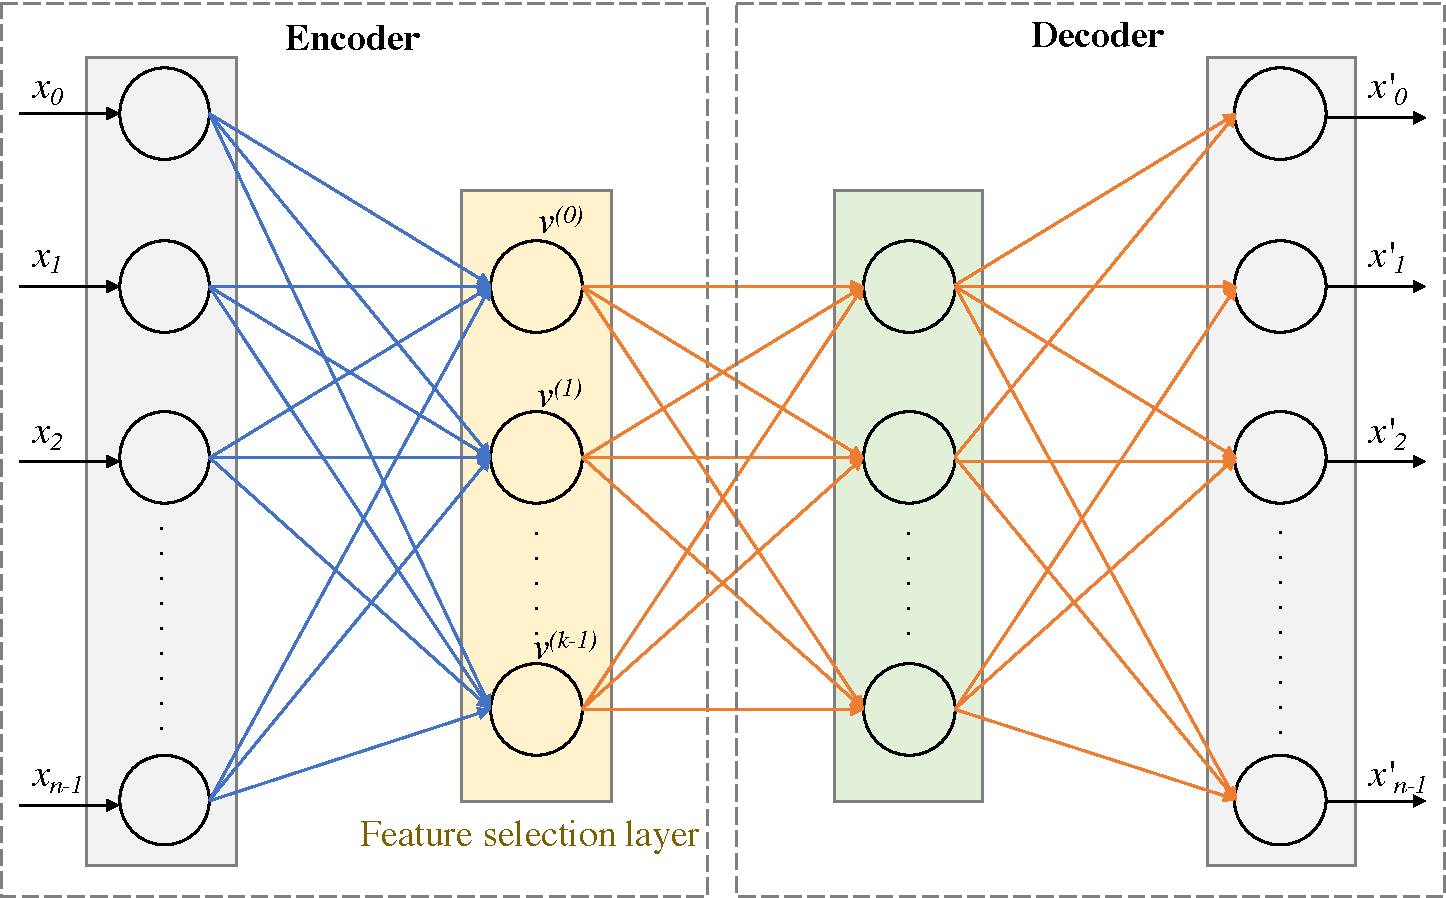
\includegraphics[scale=0.5]{fig/architecture.pdf}
    \caption{\textbf{Architecture of Concrete Relaxation Autoencoder.} Proposed feature selection architecture is consists of a encoder and a decoder. The layer after input layer in encoder is called concrete feature selection layer shown in yellow. This layer has k number of node where each node is for each feature to be selected. During the training stage, the $i^{th}$ node $u^{(i)}$ takes the value $x^Tm^{(i)}$.
During testing stage, these weights are fixed and the element with the highest value is selected by the corresponding $i^{th}$ hidden node.
The architecture of the decoder remains the same during train and test stage.}
    \label{fig:architecture}
\end{figure*}


We use Concrete relaxation discrete random variables to select input features in
the following way. For each of the $k$ nodes in the concrete
selector layer, we sample a $d-$dimensional Concrete random
variable $m^{(i)}, i \in { 1....k}$ (note that the superscript here
indexes the node in the selector layer, whereas the subscript
earlier referred to the element in the vector). The $i^{th}$ node in
the selector layer $u^{(i)}$ outputs $x . m^{(i)}$. This is, in general, a
weighted linear combination of the input features, but notice
that when $T \to 0$, each node in the concrete selector layer
outputs exactly one of the input features. After the network
is trained, during test time, we thus replace the concrete
selector layer with a discrete arg max layer in which the
output of the $i^{th}$ neuron is $x_{arg-max_j \alpha _j ^(i)}$

% \subsection{Annealing Schedule}

The temperature of Concrete random variables in the concrete selector layer has a significant affect on the output
of the nodes. If the temperature is held high, the concrete
selector layer continuously outputs a linear combination of
features. On the contrary, if the temperature is held low, the
concrete selector layer is not able to explore different combinations of features and converges to a poor local minimum.
Neither fixed temperature allows the concrete selector layer
to converge to informative features.

Instead, we propose a simple annealing schedule that sets the temperature for all of the concrete variables, initially
beginning with a high temperature $T_0$ and gradually decaying the temperature until a final temperate $T_B$ at each
epoch according to a first-order exponential decay: $T(b) =
T_0(T_B/T_0)^{b/B}$ where $T(b)$ is the temperature at epoch number $b$, and $B$ is the total number of epochs. We find that this annealing schedule
allows the concrete selector layer to effectively stochastically explore combinations of features in the initial phases
of training, while in the later stages of training, the lowered
temperature allows the the network to converge to informative individual features.

\begin{figure}[hbt]
    \centering
    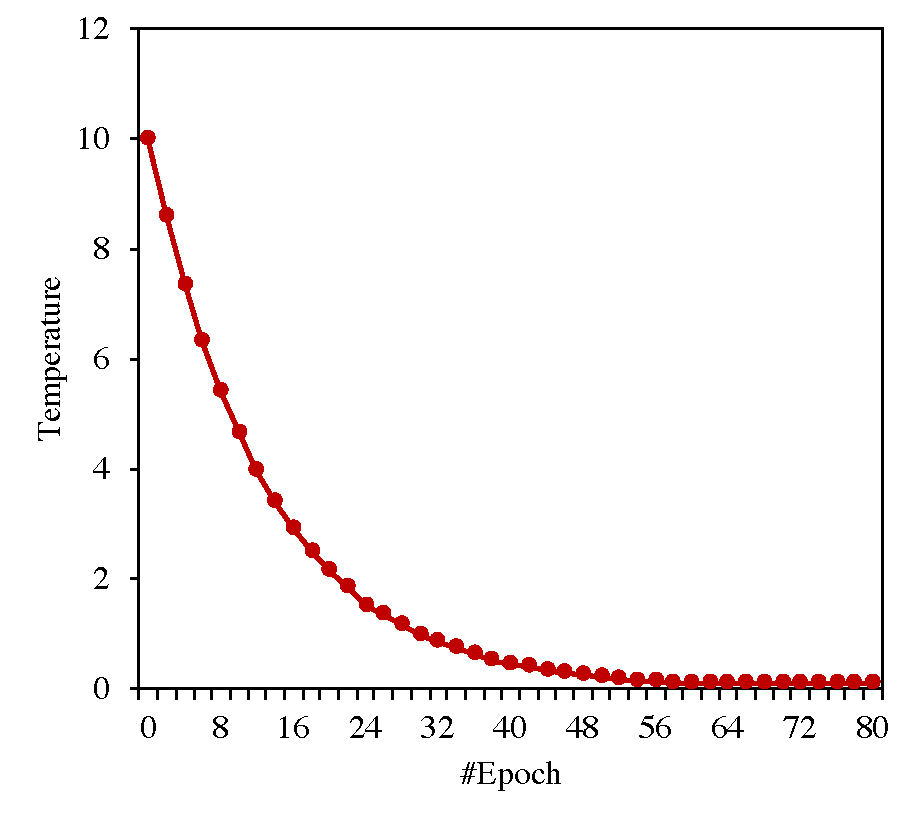
\includegraphics[scale=0.5]{fig/temp-epoch-mRNA.pdf}
    \caption{\textbf{Annealing schedules for the CoRAE.} Here, we show the effect of different annealing schedules on a
concrete autoencoder trained on the mRNA dataset with $k$ = 100
selected features. At each epoch, we plot the temperature in brown. If
the temperature is exponentially decayed (the annealing schedule
we use), the samples converge to informative features.}
    \label{fig:architecture}
\end{figure}

\subsection{Gene Selection, classification, evaluation, and validation}
Top genes are selected based on two criteria - a) classification accuracy needs to be greater than 90\% ($ \theta > 90\% $),
and b) number of genes should be as less as possible so that we can filter out only important genes. The reason of
selecting less number of genes is to provide them to any biologist so that they can conduct wet lab experiment
easily. Important genes are also selected by two state-of-the-art methods SVM-RFE and LASSO as used in [BIBM]. Towards fair comparison
with CoRAE, same number of genes has been selected by LASSO and SVM-RFE. The range of number of genes is 10 to 500
with an interval of 50. Thus, we select 10 sets of genes for each kind of RNA (mRNA, miRNA, and lncRNA) with three
methods (LASSO, SVM-RFE, and CoRAE). For parameter tuning, we used GridSearch method. Each set of gene is used for classifying 33 cancer types. SVM is used for
classification. For classification, total number of samples has been splitted into two sets: 75\% for training and
25\% for testing set. Five different evaluation metrics has been used to record the classification performance such
as accuracy, precision, recall, f1 score and MSE (mean squared error). Performance matrices are measured on the independent test
samples. Final gene set of each RNA type that showed highest performance is selected. The capabilities of selected
genes in pan-cancer classification is visually validated using unsupervised visualization technique tSNE.
%Survival analysis is conducted for testing the prognostic capabilities of selected gene set. 



\section{Result}
A series of experiements is conducted to compare the performance of CoRAE with other state-of-the-art feature selection methods such as LASSO and SVM-RFE. We have selected a range of features from 10 to 500 using all three methods then train a linear classifier (SVM) using selected coding and non-coding gene expression of 33 cancer patients. \ref{fig:acc-mse} shows the classification performance for different number of features. Across the all k, CoRAE has highest accuracy and lowest error for both mRNA and lncRNA expression. Even if the number of feature is low e.g. 10, the accuracy is almost 80\% whereas LASSO and SVM-RFE shows poor restuls for lowest number of feature. For more than 50 features, all the methods shows above 90\% accuracy. Also, CoRAE shows less error with less number of features. It starts from 38 and quickly reduced to less 10 within 50 features. The behaviour in classification is almost symetrical in both coding and non-coding genes. However, mRNA expression performs slightly better than lncRNA which is shown in \ref{fig:acc-mRNA-lncRNA.}.
\begin{figure*}[hbt]
    \centering
    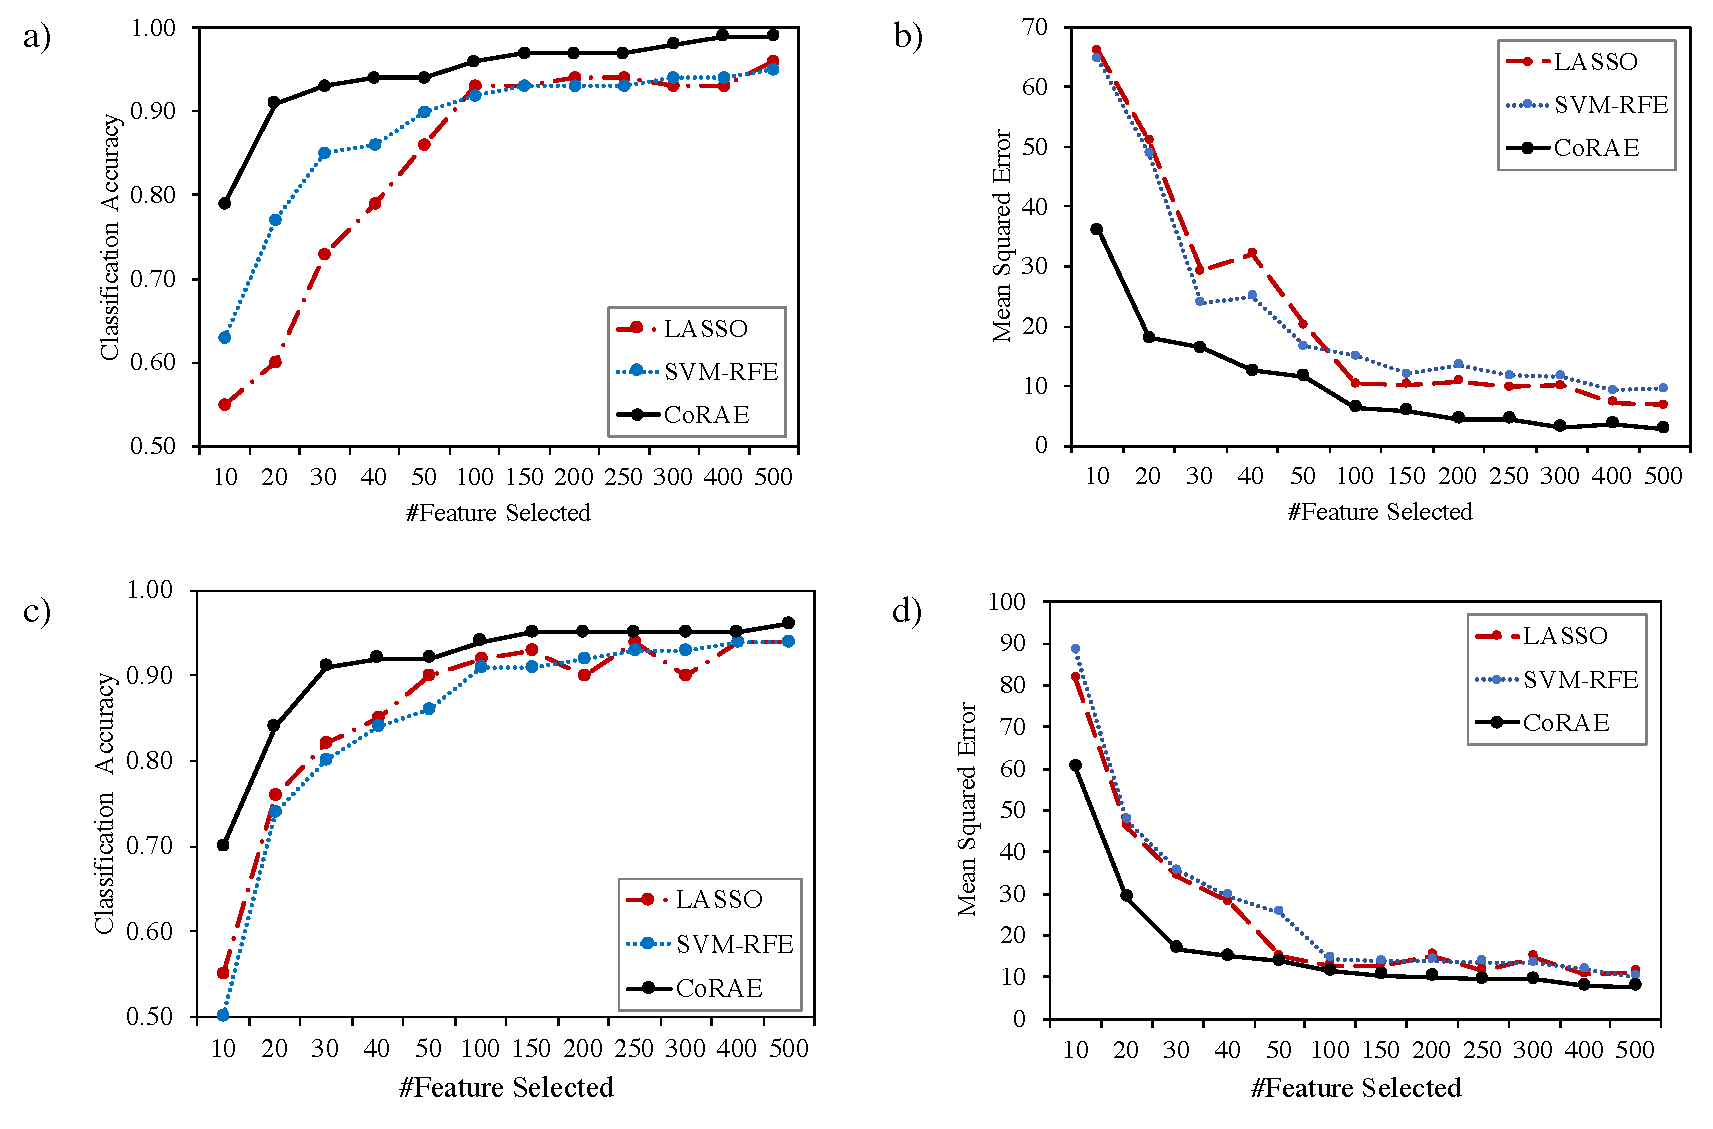
\includegraphics[scale=0.5]{fig/acc-mse.pdf}
    \caption{\textbf{Classification performance using selected RNA features.}  Comparison of CoRAE with other feature selection methods. Througout the all values of k tested on both mRNA(a) and lncRNA(c) CoRAE have highest classifcation accuracy. Similarly, it shows lowest mean squared error on both mRNA(b) and lncRNA(d)}
    \label{fig:acc-mse}
\end{figure*}

\begin{figure}[hbt]
    \centering
    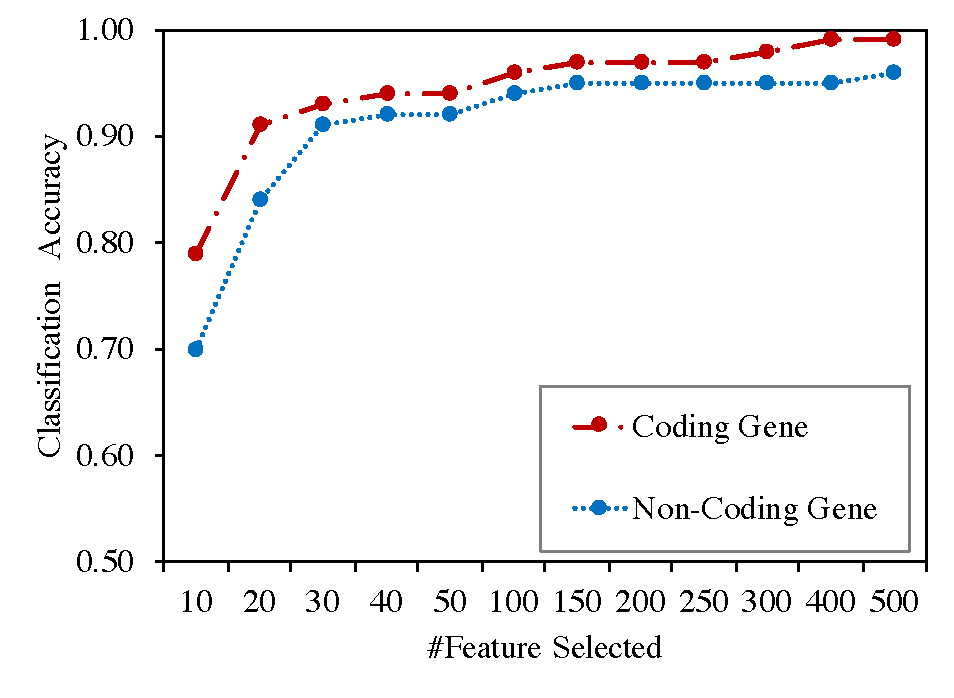
\includegraphics[scale=0.6]{fig/acc-mRNA-lncRNA.pdf}
    \caption{\textbf{Classification accuracy comparison between coding and non-coding genes expression.} Across all the $k$, mRNA expression shows slightly better classification accuracy over lncRNA expression. Here, these features has been seelcted using proposed method only.}
    \label{fig:acc-mRNA-lncRNA.}
\end{figure}

\begin{figure*}[hbt]
    \centering
    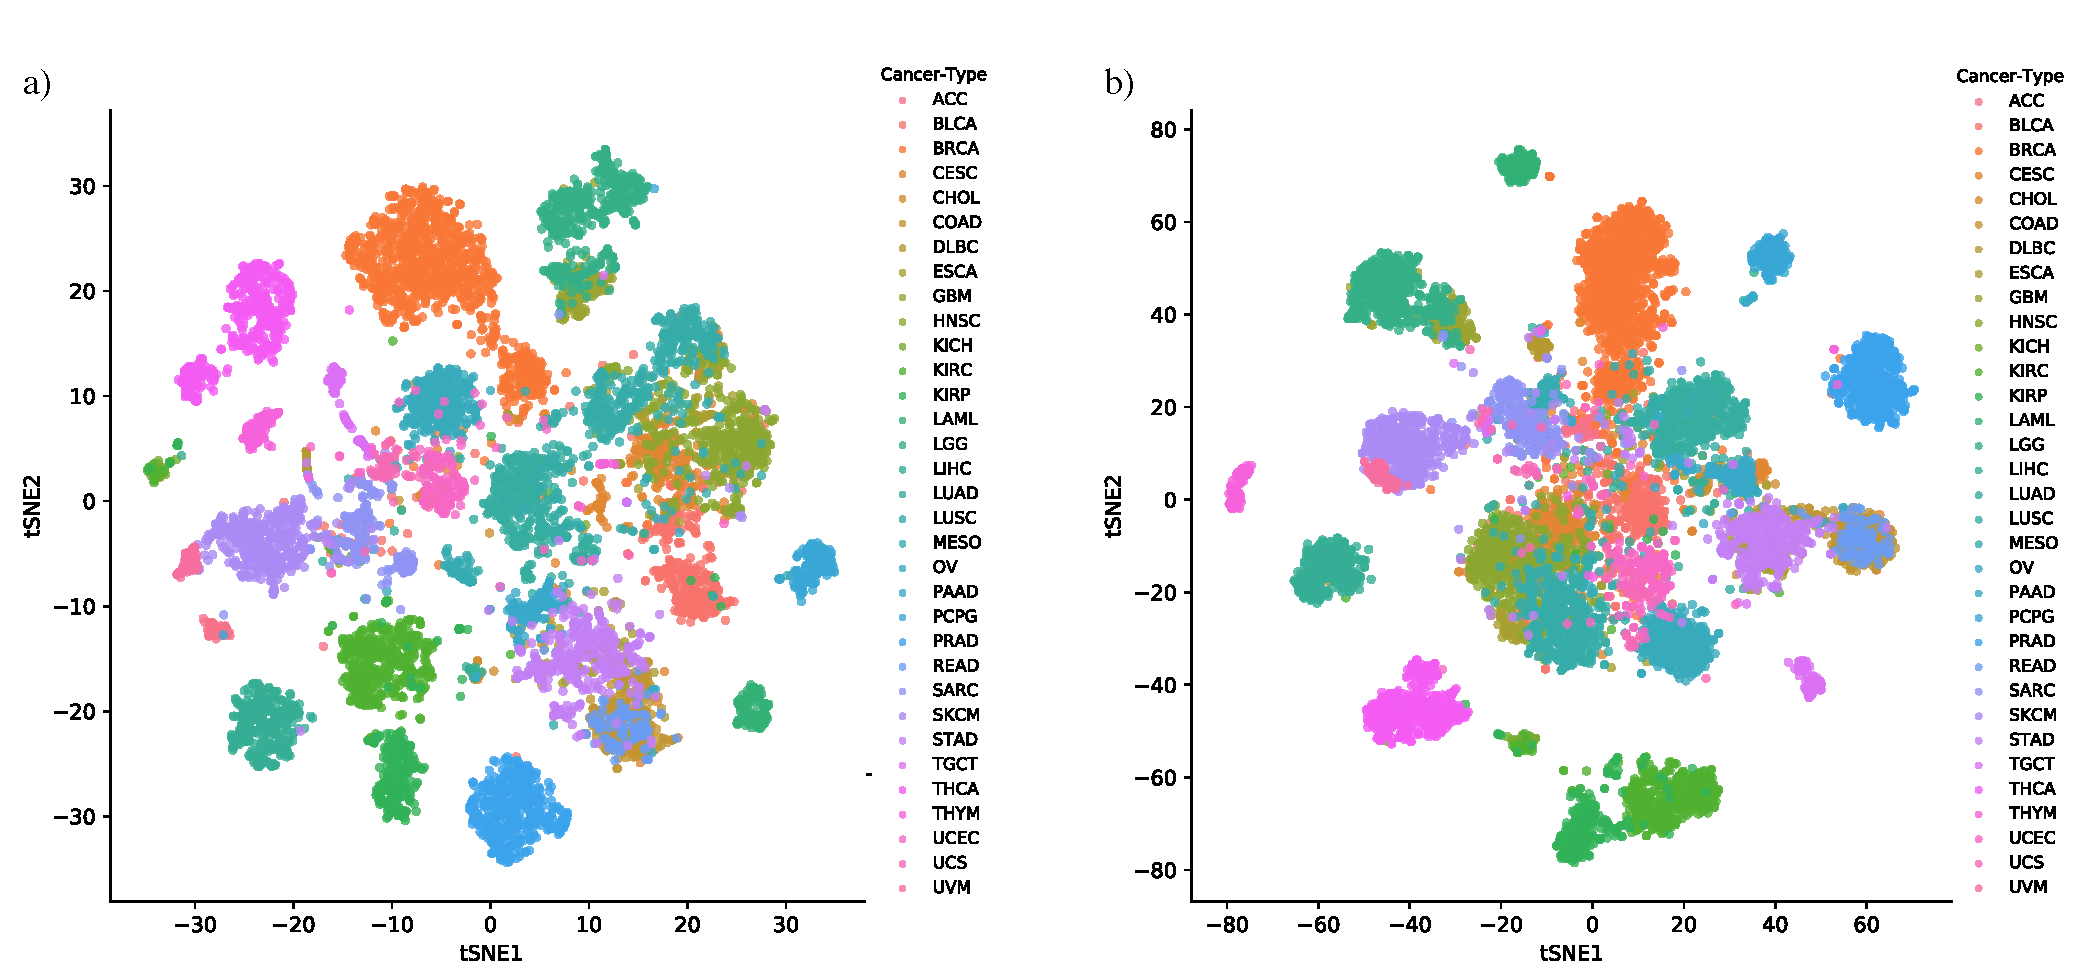
\includegraphics[scale=0.45]{fig/tSNE.pdf}
    \caption{\textbf{Visualization of 33 different cancer types using top-100 CoRAE features.} Here, we show the t-SNE representation of 33 cancer samples using selected features. Each dot represents a cancer sample and each color represents a cancer type. a) t-SNE using top 100 mRNA, b) t-SNE using top 100 lncRNA}
    \label{fig:tsne}
\end{figure*}



%\begin{figure}[hbt]
%    \centering
%    \includegraphics[scale=0.5]{fig/.pdf}
%    \caption{}
%    \label{fig:}
%\end{figure}
\subsection{Interpreting related features}

\section{Discussion}

\section{Conclusion}

future work: we will conduct more biological validation in our extended work such as survival analysis of 33 cancer patients using selected features to measure the prognostic capabilities. Similarly, pathway analysis of selected coding and non-coding genes will be analyzed in future work as well.

\section*{Acknowledgements}


\section*{Funding}

\bibliographystyle{natbib}
%\bibliographystyle{achemnat}
%\bibliographystyle{plainnat}
%\bibliographystyle{abbrv}
%\bibliographystyle{bioinformatics}
%
%\bibliographystyle{plain}
%
\bibliography{document}


% \begin{thebibliography}{}

% \bibitem[Bofelli {\it et~al}., 2000]{Boffelli03}
% Bofelli,F., Name2, Name3 (2003) Article title, {\it Journal Name}, {\bf 199}, 133-154.

% \bibitem[Bag {\it et~al}., 2001]{Bag01}
% Bag,M., Name2, Name3 (2001) Article title, {\it Journal Name}, {\bf 99}, 33-54.

% \bibitem[Yoo \textit{et~al}., 2003]{Yoo03}
% Yoo,M.S. \textit{et~al}. (2003) Oxidative stress regulated genes
% in nigral dopaminergic neurnol cell: correlation with the known
% pathology in Parkinson's disease. \textit{Brain Res. Mol. Brain
% Res.}, \textbf{110}(Suppl. 1), 76--84.

% \bibitem[Lehmann, 1986]{Leh86}
% Lehmann,E.L. (1986) Chapter title. \textit{Book Title}. Vol.~1, 2nd edn. Springer-Verlag, New York.

% \bibitem[Crenshaw and Jones, 2003]{Cre03}
% Crenshaw, B.,III, and Jones, W.B.,Jr (2003) The future of clinical
% cancer management: one tumor, one chip. \textit{Bioinformatics},
% doi:10.1093/bioinformatics/btn000.

% \bibitem[Auhtor \textit{et~al}. (2000)]{Aut00}
% Auhtor,A.B. \textit{et~al}. (2000) Chapter title. In Smith, A.C.
% (ed.), \textit{Book Title}, 2nd edn. Publisher, Location, Vol. 1, pp.
% ???--???.

% \bibitem[Bardet, 1920]{Bar20}
% Bardet, G. (1920) Sur un syndrome d'obesite infantile avec
% polydactylie et retinite pigmentaire (contribution a l'etude des
% formes cliniques de l'obesite hypophysaire). PhD Thesis, name of
% institution, Paris, France.

% \end{thebibliography}
\end{document}
